\section{Results}\label{sec:results}
Below are the results for the different test cases. The layout should be pretty
similar so they should be quite easy to follow.

\subsection{Test Case 1}\label{sec:test-case-1}
In this test we are testing STDM with the test case
\textit{izzy-train1.dat}.
\subsubsection{EA Parameters}\label{sec:test-case-1-parameters}
\begin{lstlisting}[frame=single, language=bash, caption=Command-line to
replicate the results]
python src/main.py 350 5 50 --mutation=0.1 --cross_rate=0.8 full_generational
tournament --k=5 --elite=3 stdm convert_neuron neuron_plot training\
data/izzy-train1.dat --bits_per_num=35 --e=0.02
\end{lstlisting}
\begin{table}[h]
	\begin{tabular}{c c}
		Variable & Value \\
		\hline
		Generations & 350 \\
		\hline
		Population size & 50 \\
		\hline
		Mutation rate & 0.1 \\
		\hline
		Crossover rate & 0.8 \\
		\hline
		Protocol & Full generational replacement \\
		\hline
		Mechanism & Tournament selection, k=5 and e=0.02 \\
		\hline
		Elitism & 3 \\
		\hline
		Bits per number & 35 \\
	\end{tabular}
	\caption{EA parameters for test case 1}
\end{table}
\subsubsection{End Results}\label{sec:test-case-1-results}
\begin{table}[h]
	\begin{tabular}{c c c c c}
		a & b & c & d & k \\
		\hline
		0.0323 & 0.0441 & -50.924 & 1.1294 & 0.0412
	\end{tabular}
	\caption{The neuron variables which gave the best solution for test case
	1}
\end{table}
\begin{figure}[h]
	\centering
	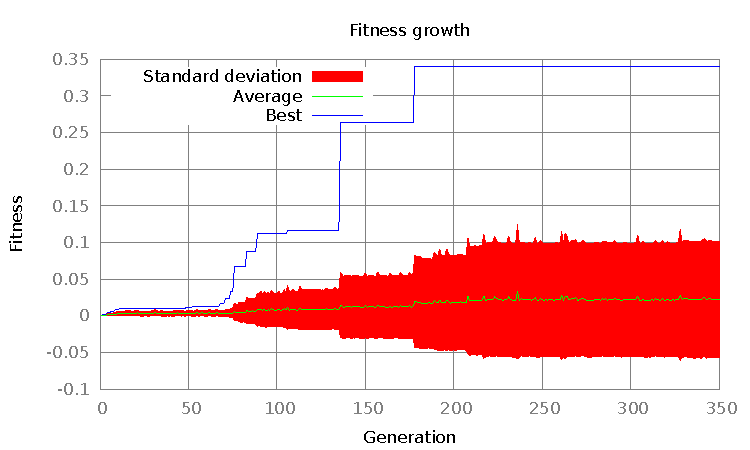
\includegraphics{../output/stdm_izzy_1_fitness.pdf}
	\caption{Fitness progression for test case 1}
	\label{fig:fitness-test-case-1}
\end{figure}
\begin{figure}[h]
	\centering
	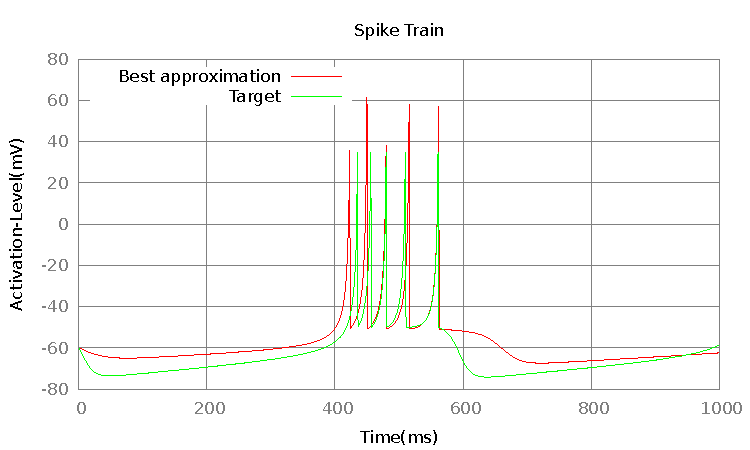
\includegraphics{../output/stdm_izzy_1_spike.pdf}
	\caption{Spike train comparison for test case 1}
	\label{fig:spike-test-case-1}
\end{figure}

\subsection{Test Case 2}\label{sec:test-case-2}
In this test we are testing SIDM with the test case
\textit{izzy-train1.dat}.
\subsubsection{EA Parameters}\label{sec:test-case-2-parameters}
\begin{table}
	\begin{tabular}{c c}
		Variable & Value \\
		\hline
		Generations & X \\
		\hline
		Population size & X \\
		\hline
		Mutation rate & X \\
		\hline
		Crossover rate & X \\
		\hline
		Protocol & X \\
		\hline
		Mechanism & X \\
		\hline
		Elitism & X \\
		\hline
		Bits per number & \\
	\end{tabular}
	\caption{EA parameters for test case 2}
\end{table}
\subsubsection{End Results}\label{sec:test-case-2-results}
\begin{table}
	\begin{tabular}{c c c c c}
		a & b & c & d & k \\
	\end{tabular}
\end{table}

\subsection{Test Case 3}\label{sec:test-case-3}
In this test we are testing WDM with the test case
\textit{izzy-train1.dat}.
\subsubsection{EA Parameters}\label{sec:test-case-3-parameters}
\begin{table}
	\begin{tabular}{c c}
		Variable & Value \\
		\hline
		Generations & X \\
		\hline
		Population size & X \\
		\hline
		Mutation rate & X \\
		\hline
		Crossover rate & X \\
		\hline
		Protocol & X \\
		\hline
		Mechanism & X \\
		\hline
		Elitism & X \\
		\hline
		Bits per number & \\
	\end{tabular}
	\caption{EA parameters for test case 3}
\end{table}
\subsubsection{End Results}\label{sec:test-case-3-results}
\begin{table}
	\begin{tabular}{c c c c c}
		a & b & c & d & k \\
	\end{tabular}
\end{table}

\subsection{Test Case 4}\label{sec:test-case-4}
In this test we are testing STDM with the test case
\textit{izzy-train2.dat}.
\subsubsection{EA Parameters}\label{sec:test-case-4-parameters}
\begin{table}
	\begin{tabular}{c c}
		Variable & Value \\
		\hline
		Generations & X \\
		\hline
		Population size & X \\
		\hline
		Mutation rate & X \\
		\hline
		Crossover rate & X \\
		\hline
		Protocol & X \\
		\hline
		Mechanism & X \\
		\hline
		Elitism & X \\
		\hline
		Bits per number & \\
	\end{tabular}
	\caption{EA parameters for test case 4}
\end{table}
\subsubsection{End Results}\label{sec:test-case-4-results}
\begin{table}
	\begin{tabular}{c c c c c}
		a & b & c & d & k \\
	\end{tabular}
\end{table}

\subsection{Test Case 5}\label{sec:test-case-5}
In this test we are testing SIDM with the test case
\textit{izzy-train2.dat}.
\subsubsection{EA Parameters}\label{sec:test-case-5-parameters}
\begin{table}
	\begin{tabular}{c c}
		Variable & Value \\
		\hline
		Generations & X \\
		\hline
		Population size & X \\
		\hline
		Mutation rate & X \\
		\hline
		Crossover rate & X \\
		\hline
		Protocol & X \\
		\hline
		Mechanism & X \\
		\hline
		Elitism & X \\
		\hline
		Bits per number & \\
	\end{tabular}
	\caption{EA parameters for test case 5}
\end{table}
\subsubsection{End Results}\label{sec:test-case-5-results}
\begin{table}
	\begin{tabular}{c c c c c}
		a & b & c & d & k \\
	\end{tabular}
\end{table}

\subsection{Test Case 6}\label{sec:test-case-6}
In this test we are testing WDM with the test case
\textit{izzy-train2.dat}.
\subsubsection{EA Parameters}\label{sec:test-case-6-parameters}
\begin{table}
	\begin{tabular}{c c}
		Variable & Value \\
		\hline
		Generations & X \\
		\hline
		Population size & X \\
		\hline
		Mutation rate & X \\
		\hline
		Crossover rate & X \\
		\hline
		Protocol & X \\
		\hline
		Mechanism & X \\
		\hline
		Elitism & X \\
		\hline
		Bits per number & \\
	\end{tabular}
	\caption{EA parameters for test case 6}
\end{table}
\subsubsection{End Results}\label{sec:test-case-6-results}
\begin{table}
	\begin{tabular}{c c c c c}
		a & b & c & d & k \\
	\end{tabular}
\end{table}

\subsection{Test Case 7}\label{sec:test-case-7}
In this test we are testing STDM with the test case
\textit{izzy-train3.dat}.
\subsubsection{EA Parameters}\label{sec:test-case-7-parameters}
\begin{table}
	\begin{tabular}{c c}
		Variable & Value \\
		\hline
		Generations & X \\
		\hline
		Population size & X \\
		\hline
		Mutation rate & X \\
		\hline
		Crossover rate & X \\
		\hline
		Protocol & X \\
		\hline
		Mechanism & X \\
		\hline
		Elitism & X \\
		\hline
		Bits per number & \\
	\end{tabular}
	\caption{EA parameters for test case 7}
\end{table}
\subsubsection{End Results}\label{sec:test-case-7-results}
\begin{table}
	\begin{tabular}{c c c c c}
		a & b & c & d & k \\
	\end{tabular}
\end{table}

\subsection{Test Case 8}\label{sec:test-case-8}
In this test we are testing SIDM with the test case
\textit{izzy-train3.dat}.
\subsubsection{EA Parameters}\label{sec:test-case-8-parameters}
\begin{table}
	\begin{tabular}{c c}
		Variable & Value \\
		\hline
		Generations & X \\
		\hline
		Population size & X \\
		\hline
		Mutation rate & X \\
		\hline
		Crossover rate & X \\
		\hline
		Protocol & X \\
		\hline
		Mechanism & X \\
		\hline
		Elitism & X \\
		\hline
		Bits per number & \\
	\end{tabular}
	\caption{EA parameters for test case 8}
\end{table}
\subsubsection{End Results}\label{sec:test-case-8-results}
\begin{table}
	\begin{tabular}{c c c c c}
		a & b & c & d & k \\
	\end{tabular}
\end{table}

\subsection{Test Case 9}\label{sec:test-case-9}
In this test we are testing WDM with the test case
\textit{izzy-train3.dat}.
\subsubsection{EA Parameters}\label{sec:test-case-9-parameters}
\begin{table}
	\begin{tabular}{c c}
		Variable & Value \\
		\hline
		Generations & X \\
		\hline
		Population size & X \\
		\hline
		Mutation rate & X \\
		\hline
		Crossover rate & X \\
		\hline
		Protocol & X \\
		\hline
		Mechanism & X \\
		\hline
		Elitism & X \\
		\hline
		Bits per number & \\
	\end{tabular}
	\caption{EA parameters for test case 9}
\end{table}
\subsubsection{End Results}\label{sec:test-case-9-results}
\begin{table}
	\begin{tabular}{c c c c c}
		a & b & c & d & k \\
	\end{tabular}
\end{table}

\subsection{Test Case 10}\label{sec:test-case-10}
In this test we are testing STDM with the test case
\textit{izzy-train4.dat}.
\subsubsection{EA Parameters}\label{sec:test-case-10-parameters}
\begin{table}
	\begin{tabular}{c c}
		Variable & Value \\
		\hline
		Generations & X \\
		\hline
		Population size & X \\
		\hline
		Mutation rate & X \\
		\hline
		Crossover rate & X \\
		\hline
		Protocol & X \\
		\hline
		Mechanism & X \\
		\hline
		Elitism & X \\
		\hline
		Bits per number & \\
	\end{tabular}
	\caption{EA parameters for test case 10}
\end{table}
\subsubsection{End Results}\label{sec:test-case-10-results}
\begin{table}
	\begin{tabular}{c c c c c}
		a & b & c & d & k \\
	\end{tabular}
\end{table}

\subsection{Test Case 11}\label{sec:test-case-11}
In this test we are testing SIDM with the test case
\textit{izzy-train4.dat}.
\subsubsection{EA Parameters}\label{sec:test-case-11-parameters}
\begin{table}
	\begin{tabular}{c c}
		Variable & Value \\
		\hline
		Generations & X \\
		\hline
		Population size & X \\
		\hline
		Mutation rate & X \\
		\hline
		Crossover rate & X \\
		\hline
		Protocol & X \\
		\hline
		Mechanism & X \\
		\hline
		Elitism & X \\
		\hline
		Bits per number & \\
	\end{tabular}
	\caption{EA parameters for test case 11}
\end{table}
\subsubsection{End Results}\label{sec:test-case-11-results}
\begin{table}
	\begin{tabular}{c c c c c}
		a & b & c & d & k \\
	\end{tabular}
\end{table}

\subsection{Test Case 12}\label{sec:test-case-12}
In this test we are testing WDM with the test case
\textit{izzy-train4.dat}.
\subsubsection{EA Parameters}\label{sec:test-case-12-parameters}
\begin{table}
	\begin{tabular}{c c}
		Variable & Value \\
		\hline
		Generations & X \\
		\hline
		Population size & X \\
		\hline
		Mutation rate & X \\
		\hline
		Crossover rate & X \\
		\hline
		Protocol & X \\
		\hline
		Mechanism & X \\
		\hline
		Elitism & X \\
		\hline
		Bits per number & \\
	\end{tabular}
	\caption{EA parameters for test case 12}
\end{table}
\subsubsection{End Results}\label{sec:test-case-12-results}
\begin{table}
	\begin{tabular}{c c c c c}
		a & b & c & d & k \\
	\end{tabular}
\end{table}
